% ---- Writer 3 shared definitions (used by 3.6 - 3.10) ----
\tikzset{
  w3box/.style={draw,rounded corners=2pt,fill=gray!12,align=center,font=\footnotesize,minimum height=8mm,inner sep=3pt},
  w3dark/.style={draw,rounded corners=2pt,fill=gray!30,align=center,font=\footnotesize,minimum height=8mm,inner sep=3pt},
  w3store/.style={draw,fill=white,align=center,font=\footnotesize,minimum height=8mm,inner sep=3pt,double,double distance=1pt},
  w3io/.style={draw,rounded corners=6pt,fill=white,align=center,font=\footnotesize,minimum height=8mm,inner sep=3pt},
  w3dec/.style={draw,diamond,aspect=2.2,fill=white,align=center,font=\scriptsize,inner sep=1pt},
  w3arr/.style={-{Stealth[length=2.2mm]},thick},
  w3dash/.style={-{Stealth[length=2.2mm]},thick,dashed},
  w3group/.style={draw,dashed,rounded corners=4pt,inner sep=5pt},
  w3lab/.style={font=\scriptsize,inner sep=1.5pt}
}

\subsection{Style extraction and glyph library}
\label{sec:styleprofile}

This subsection describes how a writer's style is learned from photographs of that writer's pages and stored permanently (functional units FU~2.5 to FU~2.7; requirements R1 and R6).
Training a writer trains no network: a \emph{style profile} is one text file built once per writer, holding a library of that writer's own letter shapes, each reduced to a thin centre-line pen path called a \emph{glyph}, plus measured numbers such as slant, letter height, spacing and how often letters are joined, after which no page images and no networks are needed to write in that style.
The builder is an offline program written for this project which uses the recogniser of Section~\ref{sec:textrec} for inference only; its input is the line crops and transcriptions of Section~\ref{sec:segmentation}, ten pages each of the eight database writers with the last labelled page held out so that no evaluation text enters a profile, and the notebook pages of the five personal writers abhinav, dylan, owen, thiya and yeukita with 15\,\% of their lines held out.
It runs twelve stages in strict order, with no branch and no loop, and the subsections below take them in that order: a line crop and its transcript go to the recogniser for its 160 log-probability vectors; those are forced-aligned by Equation~\ref{eq:sty-viterbi}; the character territories are cut at thin low columns by Equation~\ref{eq:sty-cut}; the line is binarised, stripped of rules and thinned as a whole; the skeleton is traced into chains, spurs pruned and junctions re-joined; the chains are split at the territories and simplified; each is normalised to the x-height frame of Equation~\ref{eq:sty-norm}; the quality gates and the letter prior of Equation~\ref{eq:sty-prior} are applied; the surviving variants, the medoid and the denoised prototype are assembled; the style statistics are measured; and one JavaScript Object Notation profile per writer is written.

\subsubsection{Forced alignment: where is each character?}

To cut a letter out of a line, the builder has to know where that letter is. In joined handwriting a character has no visible boundary, and no per-character labels exist for any of the data, so the position has to be inferred. What is available is the transcript of the line and a recogniser that reads lines, and the two together are enough.

\emph{Forced alignment} is the name for using a trained recogniser backwards. Normally the recogniser is asked what the line says; here the answer is already known, and it is instead asked \emph{where} it saw each character of that known answer. The word ``forced'' refers to this: the alignment is constrained to produce the transcript that is known to be correct, so the recogniser is not permitted to decide that the line says something else. The output is an assignment of each of the $T=160$ time steps, each covering a 4-pixel slice of the line, to one character of the transcript.

The quantities involved are the transcript $y=(y_1,\ldots,y_U)$, its blank-augmented form $y'=(\varnothing,y_1,\varnothing,\ldots,y_U,\varnothing)$ of length $S=2U+1$, which is the same construction CTC uses, and the log-probabilities $\ell_t(k)=\ln y_t^k$ the recogniser produces.

The difference between this and the training loss is one operator. Where the CTC loss of Equation~\ref{eq:rec-alpha} \emph{sums} the probability over every alignment, because for training it does not matter which alignment was right, Equation~\ref{eq:sty-viterbi} takes the \emph{maximum} instead and keeps only the single most probable one, because here the alignment is precisely what is wanted. This is the Viterbi algorithm~\cite{viterbi1967}, and $\delta_t(s)$ is the log-probability of the best path that reaches position $s$ of $y'$ at step $t$:
\begin{equation}
\begin{split}
&\delta_1(1)=\ell_1(\varnothing),\quad\delta_1(2)=\ell_1(y'_2),\quad\delta_1(s)=-\infty\ (s>2),\\
&\delta_t(s)=\ell_t(y'_s)+\max\bigl\{\delta_{t-1}(s),\ \delta_{t-1}(s-1),\ \delta^{\mathrm{skip}}_{t-1}(s)\bigr\},\\
&\delta^{\mathrm{skip}}_{t-1}(s)=\begin{cases}\delta_{t-1}(s-2)&s\ge3,\ y'_s\ne\varnothing,\ y'_s\ne y'_{s-2},\\-\infty&\text{otherwise.}\end{cases}
\end{split}
\label{eq:sty-viterbi}
\end{equation}
Because the maximum replaces the sum, the path itself can be recovered. Each step records which of the three predecessors won, and following those \emph{back-pointers} backwards from the end gives the whole best path at a total cost of $O(TS)$. The path is started from whichever of the last character or the final blank ends with the higher score, and character $i$ then owns every step whose winning position is $s^*_t=2i$, the odd positions being the blanks between characters.

The alignment is only as trustworthy as the recogniser's reading of that line, so lines the recogniser never really read must be discarded before their letters enter the library. The measure used is the \emph{alignment confidence} $\mathrm{conf}=\frac1T\sum_t\ell_t(y'_{s^*_t})$, which is the mean log-probability along the chosen path. A line where the recogniser was confident at every step scores near zero, and one where it was guessing scores strongly negative. The threshold is relative rather than absolute: a line is dropped when its confidence falls below the 25th percentile of that same writer's lines, provided at least eight lines survive. A per-writer threshold is used because the absolute confidence depends on how well the recogniser handles that hand in the first place, so one fixed cut-off would discard almost everything from the most difficult writers. On writer 153 this discards 22 of 88 lines.

The recogniser input is left-aligned at the uniform scale of Equation~\ref{eq:rec-resize}, so a frame boundary converts back to a crop pixel exactly, by Equation~\ref{eq:sty-f2p},
\begin{equation}
x_{\mathrm{px}}(a)=\frac{640\,a}{T\,s},\qquad s=\min\Bigl(\frac{64}{h},\frac{640}{w}\Bigr),
\label{eq:sty-f2p}
\end{equation}
for a crop of $h\times w$ pixels, about 6 pixels per frame on a 980-pixel line.
The span a CTC model assigns to a character cannot be used directly as the letter's extent. A CTC network is free to emit a character at any one step inside its true extent and blanks elsewhere, and in practice it emits a narrow sliver that lags slightly behind the ink. The spans are therefore used only for their \emph{centres} $c_k$, which are reliable, and the provisional boundary between two characters is taken as the midpoint between consecutive centres, $\hat x_k=\tfrac12(c_{k-1}+c_k)$.

That midpoint is only an estimate, and cutting there would often fall in the middle of a letter. In joined writing the only place where one letter honestly ends and the next begins is the ligature, the thin connecting stroke between them, and a ligature has two measurable properties: it is \emph{thin}, carrying little ink in its column, and it is \emph{low}, sitting near the baseline rather than high in the x-height band. The cut is therefore moved to the cheapest such column within a radius $r$ of the estimate, by Equation~\ref{eq:sty-cut}:
\begin{equation}
\begin{aligned}
\mathrm{cost}(x)&=\mathrm{thin}(x)+1.15\,\mathrm{top}(x),\qquad r=\max\bigl(3,\mathrm{round}(0.5x_h)\bigr),\\
x^*&=\arg\min_{|x-\hat x_k|\le r}\Bigl[\mathrm{cost}(x)+0.6\,\frac{|x-\hat x_k|}{r}\Bigr],
\end{aligned}
\label{eq:sty-cut}
\end{equation}
The two terms of the cost are the two properties of a ligature. Here $\mathrm{thin}(x)$ is the smoothed column ink count divided by its own 60th percentile over the non-empty columns, so it is near 1 in a typical column and below 1 in a thin one, and dividing by a percentile of the line itself makes the measure independent of pen thickness. The term $\mathrm{top}(x)$ is the highest ink in that column above the baseline, measured in x-heights and limited to 3, which is large in a column containing an ascender and near zero in a column containing only a low connecting stroke. The weight of 1.15 on $\mathrm{top}$ makes height slightly more important than thinness, because a thin column high up is more likely to be the upstroke of a tall letter than a ligature. The cost is forced to zero in a column with no ink at all, since a genuine gap between two unjoined letters is always the best possible cut. The final term in $x^*$ is a penalty proportional to the distance moved, which keeps the cut near the aligned estimate when no column in range is clearly better than its neighbours. The quantity $x_h$ is the x-height of Equation~\ref{eq:wid-xh}.

Two implementation points matter. The boundaries are written into one shared array and forced to be strictly increasing, because snapping each boundary independently can move two neighbours onto the same column and leave a character with no columns at all. Figure~\ref{fig:sty-code} gives the alignment and the cut cost as pseudocode.

The cuts are vertical, not along the writer's slant, and this was a measured decision rather than an obvious one. A slanted cut follows the natural geometry of a slanted hand and seems the better choice, but glyphs cut that way do not retile cleanly when reassembled at different spacings, because each one carries a sheared edge that only matches its original neighbour. Cutting along the slant lowered writer identification of the synthesised output from 81.8\,\% to 68.6\,\%, so vertical cuts were kept.


\subsubsection{From ink to ordered pen paths}

Each line is binarised and thinned by the very functions of Section~\ref{sec:wid-strokenorm} --- the Otsu threshold~\cite{otsu1979}, the rule removal of Equation~\ref{eq:wid-rule}, the closing, the speck removal, the core band of Equation~\ref{eq:wid-xh} for the baseline and x-height, whose median over the thirteen writers ranges from 15 to 47 pixels, and the Zhang--Suen thinning~\cite{zhang1984} --- the builder importing them from the same module as the classifier.
Two things differ.
The builder keeps the one-pixel skeleton instead of re-inking it, so the constant pen width of 0.14 x-heights and its clip to 2 to 9 pixels belong to the classifier path alone; and it thins the whole line \emph{once}, before the territory cuts of Equation~\ref{eq:sty-cut} are applied to the traced centre lines, because thinning each slice separately creates a spurious spine along the cut.
The \emph{slant} is the shear that makes the strokes vertical, scored by Equation~\ref{eq:sty-slant} on the column histogram of ink pixels $(x_i,y_i)$ sheared by a trial angle $\theta$ about their mean row $\bar y$, $y$ downwards,
\begin{equation}
x'_i(\theta)=\bigl\lfloor x_i-(y_i-\bar y)\tan\theta\bigr\rfloor,\qquad H_\theta(c)=\#\{i:x'_i(\theta)=c\},\qquad S(\theta)=\sum_cH_\theta(c)^2 ,
\label{eq:sty-slant}
\end{equation}
with $\hat\theta=-\arg\max_\theta S(\theta)$ over $\theta\in\{-45^\circ,-43.5^\circ,\ldots,45^\circ\}$, forward lean positive; $\sum_cH_\theta(c)$ being fixed, the score peaks when the ink falls in the fewest columns.

A thinned image is a picture of the pen path and not yet an ordered path, and four geometric operations recover the ordering, each resting on the 8-neighbourhood degree of a skeleton pixel (Equation~\ref{eq:app-degree}): a pixel of degree one is a stroke end, of degree two an interior point, and of degree three or more a junction.
The skeleton is \emph{traced} into chains grown from each unvisited end or junction through interior pixels only, so that every skeleton pixel belongs to exactly one chain; stopping at a junction rather than choosing a branch there is what makes the decomposition unique, a junction being precisely the point at which the true pen order cannot be recovered from the image.
Short false branches left by thinning are \emph{pruned} as spurs when a chain is both shorter than 2.5 pixels and has a free end (Equation~\ref{eq:app-spur}); the conjunction is necessary, because a short chain between two \emph{two} junctions is the crossbar of an A or the waist of an e and must be kept.
Because a self-crossing stroke such as the loop of an e breaks into several chains at the junction where it crosses itself, although the pen never lifted, chain ends within 1.5 pixels are \emph{re-joined} when their outward directions are nearly opposed, the continuation test of Equation~\ref{eq:app-rejoin}, which admits the curvature a pen shows through a crossing but rejects a genuine corner.
A chain crossing a territory boundary is then split, each crossing setting $\mathrm{connL}_i$ and $\mathrm{connR}_i$ to record that the pen did not lift.
Finally each chain is \emph{simplified} by the Douglas--Peucker recursion at $\varepsilon=0.6$ pixels, 0.05 to 0.12\,mm at 4\,mm per x-height, taken from~\cite{teikari2016} where it serves the same pen-path purpose, which bounds the deviation of the stored path from the traced one by $\varepsilon$ everywhere; a closed chain must be split at its farthest vertex first, since the recursion measures distance to the line through the two ends and would otherwise collapse a loop to two points.
Appendix~\ref{sec:app-syn-trace} states all four criteria as explicit conditions, with the resampling and smoothing that remove the lattice staircase thinning leaves behind.
Equation~\ref{eq:sty-norm} then maps every simplified point $(x,y)$ of a chain in the territory $[L,R)$ into a writer-independent frame with baseline 0, $y$ up, unit x-height and the slant removed:
\begin{equation}
y_n=\frac{y_b-y}{x_h},\qquad x_n=\frac{x-L}{x_h}-\sigma\,y_n,\qquad\sigma=\tan\hat\theta .
\label{eq:sty-norm}
\end{equation}
The synthesiser applies the inverse shear of Equation~\ref{eq:syn-place}, so glyphs are stored upright and re-appear at the writer's lean.
On a side confirmed connected the outward-running low connector is trimmed, and only if 18\,\% of the glyph width remains, the entry and exit points being recorded for the synthesiser's own connector.

\subsubsection{Variants, quality gates and the cross-writer letter prior}

Of about 2\,122 to 4\,031 raw instances per writer roughly 10\,\% survive five gates applied per character in order: geometry, outliers, the cross-writer prior of Equation~\ref{eq:sty-prior}, consensus against that writer's other instances of the same letter, and typicality, which keeps the best 12.
The cascade is ordered cheapest-first and most-local-first, so that a glyph is compared with its peers only once it is known to be a plausible letter at all; Appendix~\ref{sec:app-syn} states the test each gate applies and the thresholds it uses.

The hardest gate to design is the third, because it has to decide whether a letter is malformed, and one writer's ten pages do not contain enough examples to say what a well-formed letter looks like. Thirteen writers together do, and that is the idea the gate rests on: whatever all thirteen hands agree on must be the letter itself rather than any one writer's style.

To compare shapes they must first be reduced to numbers. Each glyph is turned into a \emph{shape descriptor} $v_g$, which is built by laying a $12\times12$ grid over the glyph's bounding box and counting how much stroke falls in each cell, giving 144 numbers. Three steps follow. The counts are \emph{damped} by taking a power below one of each, so that one cell holding a dense loop cannot dominate the comparison. They are then blurred slightly across neighbouring cells, so that a stroke falling a fraction of a cell either side of a boundary does not change the descriptor abruptly. Finally the whole vector is scaled to unit length, which removes the overall amount of ink and leaves only its distribution, so that a thick pen and a thin pen give the same descriptor for the same shape.

The reference shape $\bar v_c$ for character $c$ is the element-wise median of those descriptors over all thirteen writers, also scaled to unit length. A median is used rather than a mean so that one writer with an unusual letter form cannot pull the reference towards it. Because both vectors have unit length, their dot product is the cosine of the angle between them, which is 1 for identical distributions and smaller the more they differ. The distance of a glyph from the cross-writer reference is therefore
\begin{equation}
\mathrm{priorD}(g,c)=1-v_g\cdot\bar v_c\in[0,1],
\label{eq:sty-prior}
\end{equation}
and the 70\,\% of each writer's variants with the smallest $\mathrm{priorD}$ are kept. The important property of Equation~\ref{eq:sty-prior} is the direction in which it is used. It only ever \emph{rejects} one of the writer's own variants; it never substitutes a shape taken from another writer, so no part of another person's handwriting can enter a profile through this gate.

What Equation~\ref{eq:sty-prior} measures is how \emph{typical} a shape is, and Section~\ref{sec:sty-faults} records the limitation that follows from this: typicality is not the same thing as legibility, and a writer whose letters are consistently unusual scores badly on a prior built from everyone else.

Two further glyphs are derived per character and stored alongside the variants. The \emph{medoid} is the one real variant whose total distance to all the other variants of that character is smallest, so it is the writer's most representative actual letter. A medoid is used rather than an average because an average of several curves is not itself a pen stroke, whereas a medoid is a real example the writer really wrote. The distance is measured as the sum of absolute differences between descriptors, which is the $L_1$ norm, chosen because it is less affected by one wildly different variant than a sum of squares would be. The \emph{denoised prototype} is the per-stroke median curve of the largest group of variants sharing the same stroke count, and it is prepended to the list only when it is clearly cleaner than the variants it summarises (Figure~\ref{fig:sty-glyphs}). The medoid is also what Section~\ref{sec:synthesis} uses as the \emph{anchor}, the legible stand-in drawn when a writer's own variant is judged too malformed to use.

\begin{figure}[!htbp]
\centering
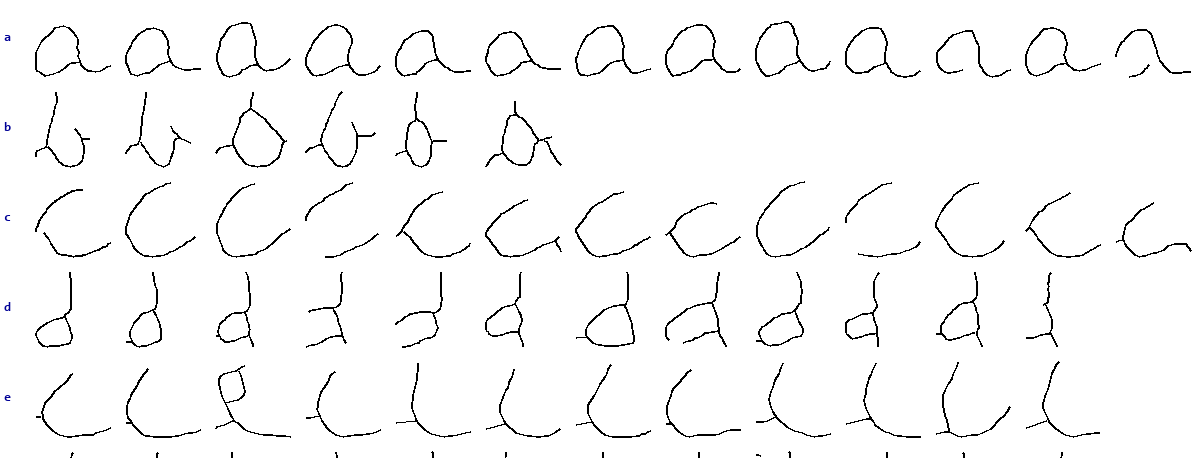
\includegraphics[width=0.78\linewidth]{Figures/w3_glyphs153_ae.png}
\caption{Stored variants of the letters a, b, c, d and e of writer 153, a strongly joined hand; each row is one character with up to 12 variants, and the short tails at the sides are remains of ligatures.}
\label{fig:sty-glyphs}
\end{figure}

\subsubsection{Style statistics and permanent storage}

Besides glyphs the profile holds numbers measured over the kept lines, every key of which is listed with an example as Table~\ref{tab:sty-schema} in Appendix~\ref{sec:app-syn}; two are not simple medians, the \emph{connectedness} being the adjacent letter pairs whose $\mathrm{connR}$ flag was set over all adjacent pairs, so its numerator counts the pen-down crossings recorded during tracing, and the word gap being the median of ink-free column runs wider than $0.5x_h$ on the \emph{real} ink, because CTC gives a space only a narrow slice.
Table~\ref{tab:sty-writers} shows how widely the thirteen differ --- slant $-10.5^\circ$ to $42.0^\circ$, connectedness 0.195 to 0.968, word gap 0.94 to 2.68 x-heights --- which is the diversity requirement R1 asks the system to reproduce; the thirteen files total about 4.8\,MB and load when the server starts (Section~\ref{sec:system}), which with the web interface listing them is requirement R6.
\mustdo{the demonstration of R6 (display of the stored writers, reproduction in a writer chosen by the examiner) and the storage device holding the files.}


\begin{table}[!htbp]
\centering
\fontsize{7.5}{9}\selectfont
\setlength{\tabcolsep}{2.5pt}
\begin{tabular}{|l|r|r|r|r|r|r|r|r|}
\hline
\textbf{Writer} & \textbf{Lines} & \textbf{Slant ($^\circ$)} & \textbf{$x_h$ (px)} & \textbf{$A$} & \textbf{$D$} & \textbf{Gap} & \textbf{Conn.} & \textbf{$\lambda$} \\
\hline
150 & 61 & $-4.5$ & 47 & 1.58 & $-0.72$ & 1.33 & 0.343 & 0.90$^\dagger$ \\
151 & 58 & 33.0 & 22 & 2.69 & $-1.09$ & 1.59 & 0.968 & 1.00$^\dagger$ \\
152 & 59 & 19.5 & 46 & 1.48 & $-0.79$ & 1.47 & 0.715 & 0.45$^\dagger$ \\
153 & 66 & 30.0 & 33 & 1.59 & $-1.10$ & 1.59 & 0.961 & 0.45$^\dagger$ \\
384 & 54 & 4.5 & 43 & 1.93 & $-0.71$ & 1.37 & 0.500 & 0.30$^\dagger$ \\
551 & 58 & 42.0 & 20 & 1.84 & $-0.67$ & 2.68 & 0.557 & 1.00$^\dagger$ \\
552 & 47 & $-10.5$ & 32 & 1.62 & $-0.56$ & 1.53 & 0.609 & 0.00$^\dagger$ \\
588 & 58 & 0.0 & 29 & 1.73 & $-0.68$ & 2.07 & 0.668 & 0.30$^\dagger$ \\
abhinav & 130 & 6.0 & 28 & 1.78 & $-0.84$ & 2.13 & 0.789 & --- \\
dylan & 79 & $-6.0$ & 26 & 1.68 & $-0.62$ & 1.79 & 0.195 & 1.00$^\dagger$ \\
owen & 93 & 0.0 & 32 & 1.51 & $-0.68$ & 1.10 & 0.319 & --- \\
thiya & 48 & 30.75 & 15 & 2.24 & $-1.00$ & 1.65 & 0.962 & --- \\
yeukita & 74 & 0.0 & 27 & 1.45 & $-0.58$ & 0.94 & 0.417 & 0.15$^\dagger$ \\
\hline
\end{tabular}
\caption{Scalar values of the thirteen stored style profiles, read directly from the files in \texttt{Software/CNN/NOGIT/StyleProfiles10}: kept lines, slant, pixel x-height, ascender $A$, descender $D$ and word gap (x-heights), connectedness and legibility parameter $\lambda$. Writers 150 to 588 are database writers, the last five personal. $^\dagger$The $\lambda$ column is \emph{not} read from these files, in which \texttt{legibilityLambda} is absent; it is the output of an earlier tuning run, as item~3 of Section~\ref{sec:sty-faults} records.}
\label{tab:sty-writers}
\end{table}

\subsubsection{Design alternatives and justification}

Character boundaries could have come from fixed widths, projection minima or hand labelling, but joined letters have no gaps and hand labelling of about 90 pages is impractical, while the recogniser already knows the text; several variants per letter are kept rather than one averaged letter, because averaging blurs letters whose strokes are arranged differently; and a generator learned from on-line pen data was not possible, since no such data exist for the thirteen writers, who contribute 47 to 130 usable lines each, and the pen path has to be recovered from the image in any case.
\mustdo{a figure of the builder stages on real lines: grey crop, ink mask with rules removed and core band, skeleton, traced chains in colour with the territory cuts as vertical lines, and one extracted glyph in the normalised frame, for one database and one personal line.}

\subsubsection{Known faults and limitations}
\label{sec:sty-faults}

\begin{enumerate}\setlength{\itemsep}{0pt}\setlength{\parskip}{0pt}
\item \emph{The builder cannot at present extract glyphs from a page image.} \texttt{ExtractLineGlyphs} of \texttt{BuildStyleProfile.py} opens with \texttt{from TrainText import FrameXToPixel,\,INPUT\_WIDTH}, and the delivered \texttt{TrainText.py} defines no such name in any spelling; the conversion of Equation~\ref{eq:sty-f2p} survives only as \texttt{frame\_x\_to\_pixel} in the retired tree \texttt{Software/CNN/TrainText.py}. Because the statement sits inside the function the module still imports and every cached rebuild still works, but a fresh extraction raises \texttt{ImportError} at the first line, so \emph{no new writer can be added and none of the thirteen stored profiles can at present be regenerated from the page images}.
\mustdo{repair the import in \texttt{ExtractLineGlyphs} --- either port \texttt{frame\_x\_to\_pixel} from \texttt{Software/CNN/TrainText.py} into the delivered \texttt{TrainText.py} or compute the conversion of Equation~\ref{eq:sty-f2p} in place --- then re-run the builder on all thirteen writers and confirm that the regenerated profiles match the stored ones.}
\item \texttt{legibilityLambda} is written after the build by the tuner \texttt{TuneLegibility} of \texttt{Evaluate.py} and not by the builder, and \emph{the key is absent from all thirteen files as delivered}, the profiles having been rebuilt after the tuner last ran. The server calls \texttt{SynthesizeJointBestOf}, which takes \texttt{profile.get('legibilityLambda',\,0.0)}, so \emph{the delivered system synthesises every writer at $\lambda=0$}, entirely from the writer's own glyphs with no anchor substitution at all; the older \texttt{SynthesizeLegible} falls back to 0.65 instead but is not used.
\mustdo{re-run \texttt{TuneLegibility} over the thirteen current profiles so that \texttt{legibilityLambda} is written back into each file, then re-measure the figures of Table~\ref{tab:syn-evid} that depend on it; until this is done the per-writer legibility control described in Section~\ref{sec:synthesis} is inactive.}
\item The $\lambda$ column of Table~\ref{tab:sty-writers} is a genuine measurement of that superseded run, but it describes neither the stored profiles nor the delivered system, and abhinav, owen and thiya were added afterwards and never tuned at all; the $\lambda$ gains claimed in Section~\ref{sec:synthesis} are not realised by the submitted code.
\item The stored profiles are dated 10 October 2026 and predate the current code, so the values in Tables~\ref{tab:sty-schema} and~\ref{tab:sty-writers} had to be re-read from the files rather than regenerated.
\item Cutting a joined line destroys how a letter changes with its neighbours, which is why writers 151 and 551 are reproduced least legibly (Section~\ref{sec:synthesis}).
\item The vertical-cut decision rests on a design-stage measurement, 81.8\,\% against 68.6\,\%, for which no raw log was kept.
\item The grey-level reference statistics \texttt{inkFracRef}, \texttt{aspectRef}, \texttt{paperLevel}, \texttt{inkLevel} and \texttt{midFracRef} are stored but ignored by every consumer while the pen width is constant.
\end{enumerate}
